%\documentclass[12pt]{article}
%\usepackage[margin=1 in, head=0.9 in]{geometry}
%\usepackage{fancyhdr}
%\usepackage{listings}
%\usepackage{caption}
%\usepackage{color}
%\usepackage{xcolor}
%\usepackage{caption, apacite}
%\DeclareCaptionFont{white}{\color{white}}
%\DeclareCaptionFormat{listing}{\colorbox{gray}{\parbox{\textwidth}{#1#2#3}}}
%\captionsetup[lstlisting]{format=listing,labelfont=white,textfont=white}
%\usepackage{graphicx}
%\usepackage{amsmath, amssymb, amsthm}
%\usepackage[all,cmtip]{xy}
%\pagestyle{fancy}
\input{/home/dmitry/Work/Research/thesis/FINALE/settings.tex}

%\newcommand{\ib}[1]{\bar{#1}}
%\newcommand{\ip}[1]{#1^{\prime}}
%\newcommand{\iti}[1]{\tilde{#1}}
%\newcommand{\pder}[2][]{\frac{\partial #1}{\partial #2}}
%\newcommand{\pderr}[3][]{\frac{\partial^2 #1}{\partial #2 \partial #3}}
%\newcommand{\ap}[1]{\langle #1 \rangle}
%\newcommand{\hx}[2][]{ \hat{#1}_{#2} }
%\newcommand{\hxd}[3][]{ {\hat{#1}_{{#2}_{#3}}} }
%\newcommand{\mb}[1]{\mathbf{#1}}
%\newcommand{\pp}[1]{\partial_{#1}}
%\newcommand{\vphi}{\varphi}
%\newcommand{\hqu}{\mathcal{H}}
%\newcommand{\cj}[1]{{#1}^{\star}}
%\newcommand{\rc}{\operatorname{Re}}	% complex real
%\newcommand{\ic}{\operatorname{Im}}	% complex real
\begin{document}

\title{Energy scattering of tsunami and internal tides upon interaction with bottom relief.}
\maketitle

\section*{Abstract}
The surface and interior wave motions interact with the sea bottom irregularities altering gravity wave energy propagation. Directional scattering and mode conversion will inevitably reshape a wave field and will impel restructure of localized energy budgets. Here three geophysically important cases are investigated: (1) a tsunami wave scattering from a prominent sea mount, (2) origination of a semidiurnal internal tide and (3) reflection of the internal tide from a continental slope. These problems are investigated by means of numerical experiments and theoretical analysis.\\
A tsunami wave is scattered by Koko Guoyt such that amplified and delayed signals were observed during recent tsunami events. The numerical simulations emphasize complicated response. The energy focusing occurs in dependence to tsunami incidence angel and frequencies involved. Koko guoyt as having asymmetrical shape selectively amplifies tsunami wave frequency. The provided theoretical analysis further outlines regions and parameters which would lead to higher amplification.\\
Internal tides originate from surface tide interaction with steep submarine ridges. This phenomena undergoes temporal variation leading to nonstationarity in the far field. It is shown for Tasman Sea that remote internal tide modulates magnitude of energy conversion. Further leading to spatial variability many kilometers away.\\
The Tasman Sea internal tides impinge on the continental slope partially reflecting. The reflectance markedly depends on generation of along slope leaky mode. Under some conditions coupling with the surface tide occurs leading to overall energy increase (additional source?) that outgoing energy becomes larger than incident amount. This deviates from classical two dimensional view on reflection/scattering process of the internal tides. The presented estimates of energy transfers further emphasize large variability mainly coming from along slope topography inhomogeneity.\\
Results for the problems conspicuously show importance of three dimensional topographic structure in order to describe wave energy propagation. This has strong effect on variability in the resulting wave field and wave energy sinks.

\newpage
\section{Introduction}
Oceanic gravity waves fundamentally contribute to redistribution of mechanical energy in the world ocean. The energy pathways of propagating waves can be altered in a result of interaction with large scale sea bottom features such as submarine seamountains, trenches and continental shelves. These processes appreciably shape wave propagation, and thus, leading to variation in the energy budgets. In this work, by means of numerical simulations  energy scattering of tsunamis and internal waves of tidal frequency (internal tides) is examined for cases of their interaction with ocean's bottom relief.\\
Tsunami waves are transient waves impulsively forced by submarine earthquakes and landslides. In the former case their origin lies along oceanic subduction zones such as Japan-Kuril trench (Figure 1a). These waves traversing the Pacific Ocean will encounter numerous sea bottom features. \textit{(Here let's discuss also energy decay of tsunami waves.)}\\
These open-ocean scatterers will redirect and delay wave energy creating amplified far-field signals. For example, during the Tohoku tsunami event of March, 11th 2011, tidal gauges in Northern and Central California recorded larger waves than anywhere else along the US West Coast. Notably, for some stations the secondary waves were higher than the primary.\\
Several previous studies have identified that the primary reason for the observed wave distribution is Koko Guoyt. There secondary waves originate as a result of wave scattering. This forms a distinct energy lobe (beam). Its salient feature is a bearing towards the Northern California. Additionally, trapping by Mendocino Escarpment reinforces strong tsunami waves in that region.  As it is seen, generation of the scattered waves have important consequences for forecasting of tsunami wave arrival times and post-event assessment of damage to coastal communities. This work sets its goal to develop a description for scattering mechanism at Koko Guyot.\\
% In this example, delayed waves correlated to a beam of high energy originating from a distant scatterer in Emperor seamount chain, Koko Guyot (Figure 1a). 
\begin{figure}
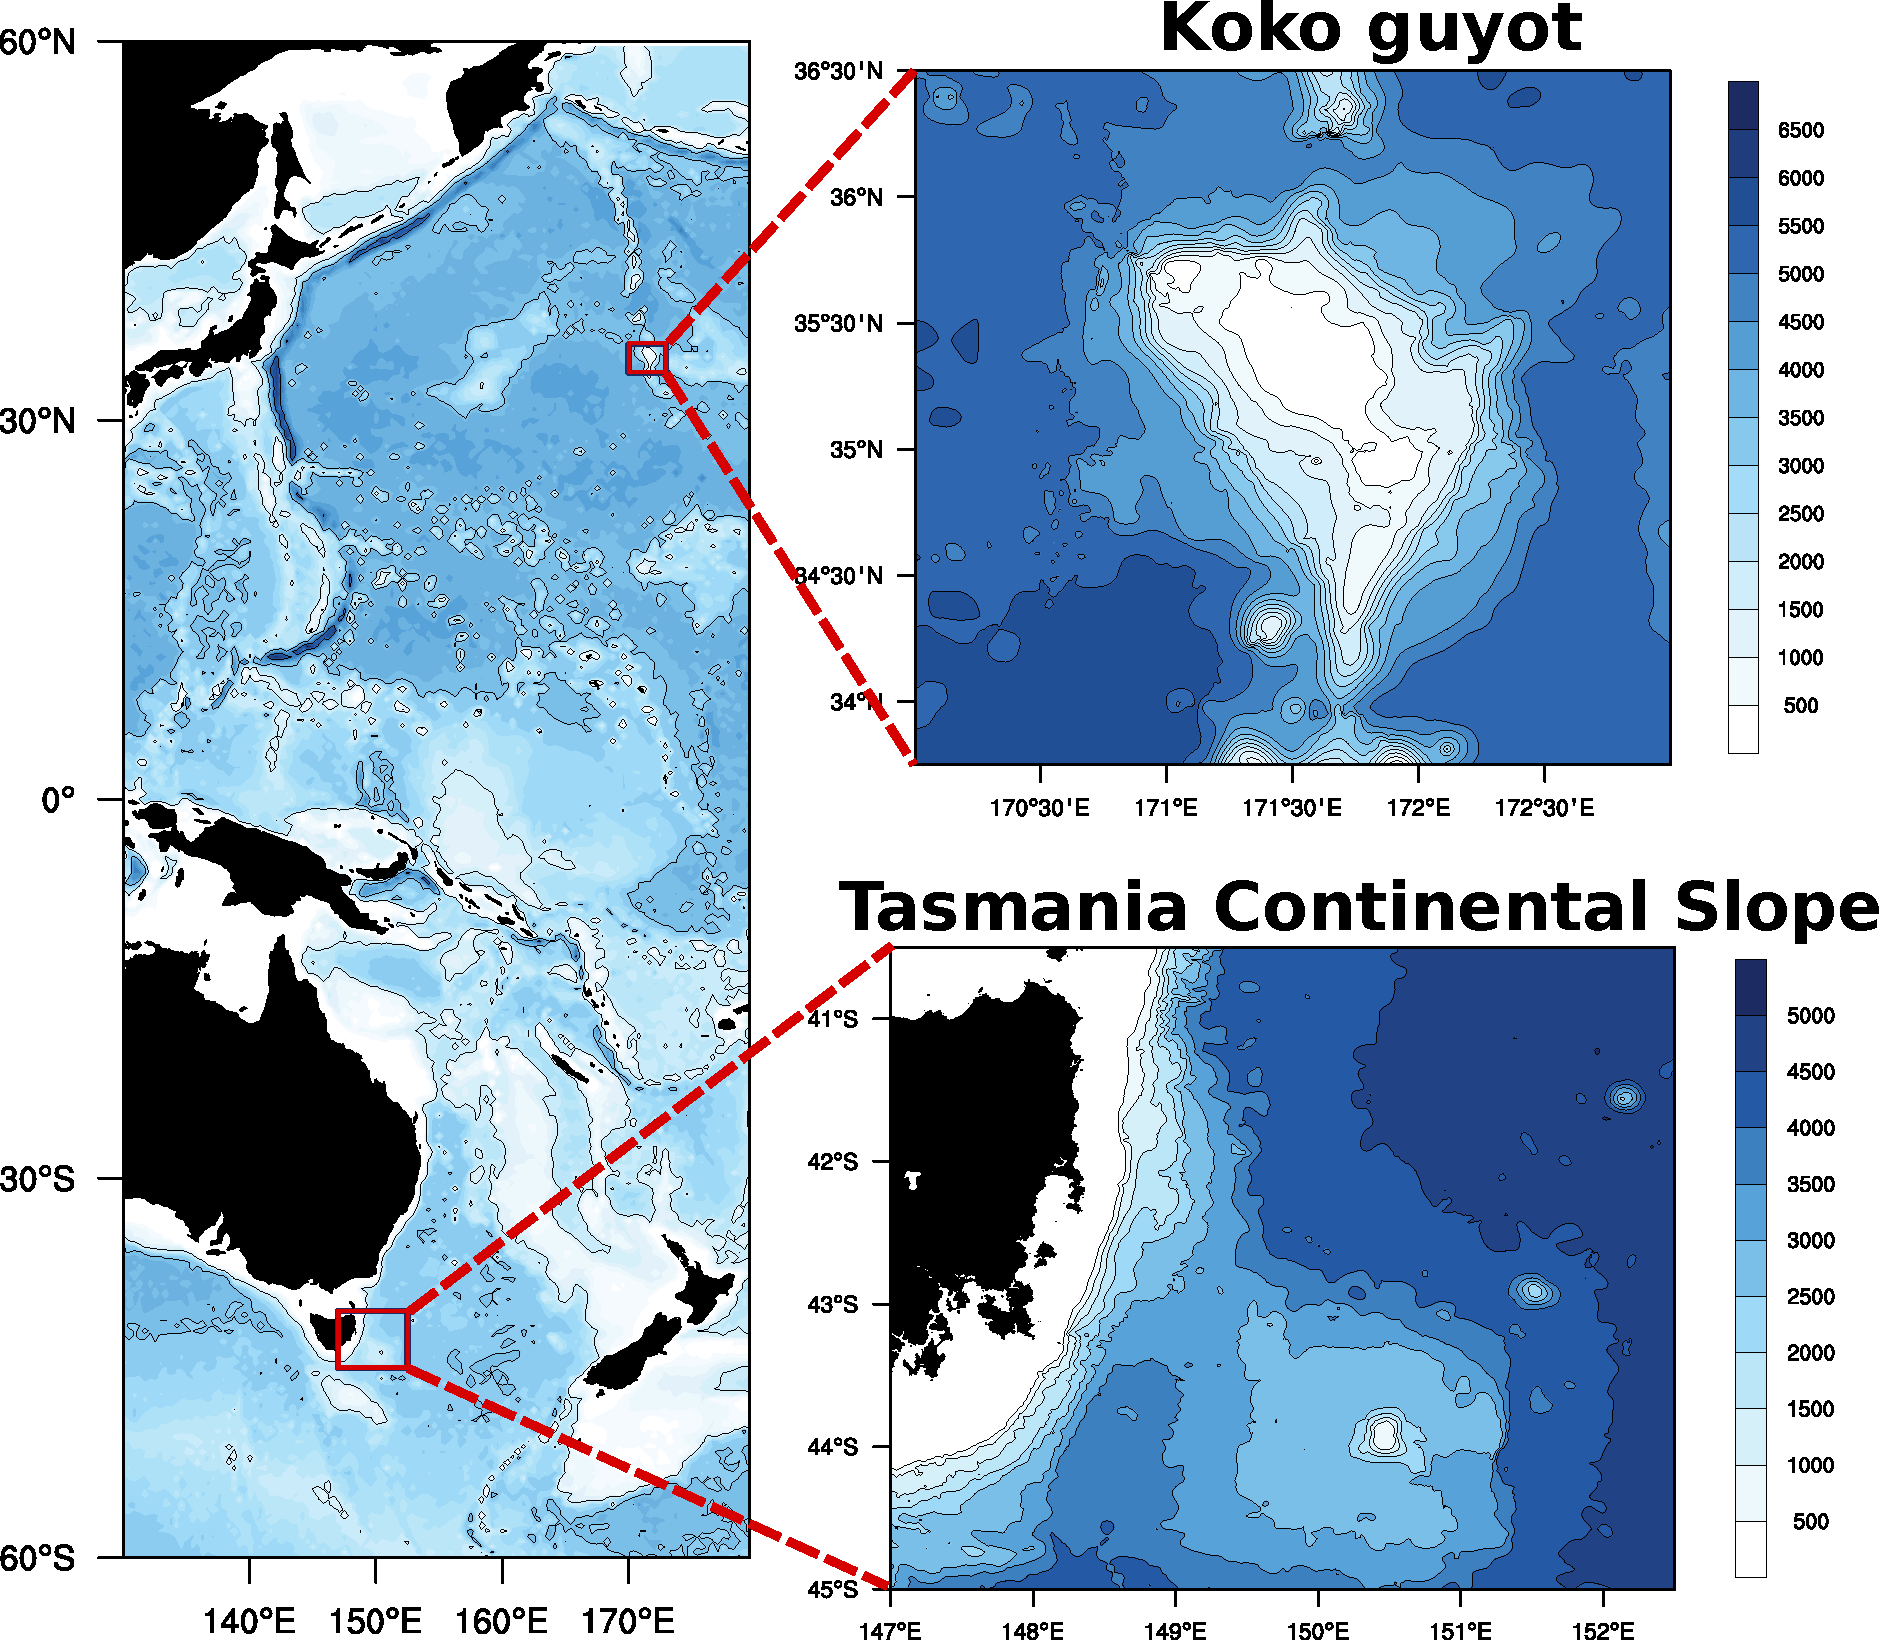
\includegraphics[scale=0.5]{../figures/map_w_places.pdf}
\caption{The map of the Pacific Ocean with outlined regions.}
\end{figure}
Wave phenomena exists through out all water column so that ocean's interior is filled with internal waves. Their existence owns to vertical stratification since the internal waves  expressed as an oscillatory motion of isopycnal surfaces. The initial perturbation can be forced by many mechanisms: wind forcing, surface buoyancy forcing, ice keels, etc. Here internal waves are caused by a tidal flow making existence of internal tides. These baroclinic waves are of tidal or quasi-tidal frequency which makes them easy to investigate.\\
The major reason for study of baroclinic tides is their non negligible role in dissipation of barotropic, surface tidal energy. Current estimates suggest that 1/3 of total tidal energy is being converted into internal motions directly in the deep ocean. Further, roughly 1/3 of that energy is lost to turbulent mixing right at generation sites while the rest emitted as freely propagating waves. These waves were observed to cross the ocean basins in form of tight beams (``spider web") without much attenuation. These observations fueled scientific research to merely (simply) understand where and how the baroclinic tidal energy is deposited. Further, since it mainly occurs deep below direct wind influence, the internal tides are thought as one of candidates for providing energy to close upwelling branch of Meridional overturning circulation.\\
In any case, characteristics of internal-tide generation, propagation and scattering are still poorly constrained. Tasman Tidal Dissipation Experiment (TTIDE) has its goal to provide some description of the phenomena in relatively simple setting of Tasman continental slope. Here an internal tidal beam originates at New Zealand, crosses Tasman Sea and impinges on the slope of Tasmania (Figure 1). The primary aim is to quantify amount of energy being reflected into the open sea.\textit{ And consequently, creating large scale understanding of internal tide reflection which allows for more describing effects of internal tides on the World Ocean.}\\
Both of the investigated geophysical problem represent a type of wave scattering by inhomogeneity in propagation media. Here, this means rapid change in ocean depth affecting wave dynamics and leading to energy scattering. Logically, an energetic approach should be taken for proper description of the latter process. The following discussion presents a  necessary dynamical background for energetic framework.\\
\textit{At such location the energy would drain into perturbations of isopycnals that further can travel hundreds of  leagues without any significant loss of energy. In the second part of my thesis origination, propagation and dissipation of the internal tidal beam is investigated on the example of Tasman Sea.\\
A global internal tide model, satellite altimetry measurements and in situ observations indicate that a ridge south of New Zealand is a site for the generation of the strong tidal beam that is directed towards the Tasman Shelf break. The low mode internal wave beam undergoes scattering from topography, which transfers energy to shorter length scales. Thus, understanding of local energy processes will lead to a more detailed picture of tidal energy dissipation.\\
\textbf{PLUGIN: 2 TW, 1 TW, Macquarie Ridge, internal tides produce transport of particulates: sediments and can cause strong currents in deep ocean. Role in tidal dissipation, Internal tides what became apparent recently are important energy transporters.}
}
\newpage

\subsection{Normal modes in flat-bottom ocean}
Tsunami and internal tides dealt in this thesis are a case of general inerto-gravity waves. And in both cases the waves are predominantly long since their typical lengthscales are order of 100 km being larger than the ocean's mean depth. Their dynamics can be well described in terms of linear and hydrostatic framework. As first step towards description of scattering phenomena, the wave propagation will be discussed for flat-bottom ocean. Than dynamics of the wave motions in stratified Boussinesq ocean with flat bottom and on a rotating f-plane (\cite{kundu2008fluid}, \cite{cushman2011introduction}) will take mathematical form of,
\begin{align}
\pder[u]{t} - f v = -\frac{1}{\ib{\rho}_0}\pder[p]{x}\\
\pder[v]{t} + f u = -\frac{1}{\ib{\rho}_0}\pder[p]{y}\\
0 = -\pder[p]{z} - \rho g\\
N^2 w = -\frac{1}{\ib{\rho}_0} \pderr[p]{z}{t}\\
\pder[u]{x} + \pder[v]{y} + \pder[w]{z} = 0
\end{align}
with $(u,~v,~w)$ being velocity along zonal, meridional and vertical axis, $f$ - Coriolis parameter, $p$ - perturbation pressure arising either from sea level oscillations or isopycnal displacements within stratified water column described by Brunt-Vaisala frequency $N^2 = -\frac{g}{\ib{\rho}_0}\pder[\rho_0]{z}$. Additionally, boundary conditions are imposed on the surface and bottom,
\begin{align}
w|_{z = 0} = \pder[\zeta]{t},~p|_{z = 0} = \ib{\rho}_0 g \zeta\\
w|_{z = -H} = 0
\end{align}
The both conditions are of linear form since the sea level motions are much smaller than acceleration due to gravity and \textit{ocean bottom is flat}. Such formulated problem allows separation of vertical axis by employing vertical mode decomposition,
\begin{align}
(u, v, p)(x,y,z,t) = \sum_{n = 0} [u_n(x,y,t), v_n(x,y,t), p_n(x,y,t)]\psi_n(z)\\
w(x,y,z,t) = \sum_{n = 0} [w_n(x,y,t)] \int_{-H}^z \psi_n(z) dz\\
\rho(x,y,z,t) = \sum_{n = 0} [\rho_n(x,y,t)] \frac{d \psi_n(z)}{dz}
\end{align}
Upon substitution of the decompositions Sturm-Liouville problem is obtained for vertical structure (basis) functions $\psi_n(z)$,
%\pder[\frac{1}{N^2 - \omega^2} \pder[\psi_n]{z}]{z} + \big(1 - \frac{f^2}{\omega^2} \big) \frac{\psi_n}{c^2_n} = 0
\begin{equation}
\frac{d}{dz}\big( \frac{1}{N^2} \frac{d \psi_n}{dz} \big) + \frac{1}{c^2_n}\psi_n = 0
\end{equation}
with an eigenvalue for a respective $n$-th vertical mode given by $c_n$ that is akin to phase speed. The carried out decomposition separates vertical motions from horizontal reducing the initial set to Laplace tidal equations,
\begin{align}
\label{In:sweq}
\begin{split}
\pder[\vec{u}_n]{t} + f \vec{k} \times \vec{u}_n = -\frac{1}{\rho_0} \nabla p_n\\
\frac{1}{\rho_0} \pder[p_n]{t} + g D_n \nabla  \cdot \vec{u}_n = 0
\end{split}
\end{align}
Here I intentionally introduced equivalent depth $D_n$ such that $c_n = \sqrt{g D_n}$. This states dynamical equivalence between barotropic (surface) wave and baroclinic (internal) waves if the ocean stratification was absent and depth was $D_n$. In actuality, $0$-th mode represents a barotropic solution with vertically uniform dynamics ($\psi_0 = const$) and equivalent depth $D_0 \simeq H$ (\cite{hendershott1981long}). This mode resembles pure surface wave propagation such as tsunami wave problem. The infinite sequence of higher vertical modes are purely internal modes that produce negligible sea level perturbations. This allows complete separation between barotropic and baroclinic motions which is similar to imposing rigid lid condition on internal modes (\cite{kundu2008fluid}).\\
Here the main interest is in linear wave phenomena, so harmonic temporal behavior $e^{i \omega t}$ will be implied leading to Helmholtz equation,
\begin{align}
\label{In:helmeq}
(\omega^2 - f^2) p_n + c_n^2 \Delta p_n = 0
\end{align}
----------------------
\begin{align}
\label{In:svw}
\begin{split}
p_n = p_{0n} e^{i \omega t - \vec{k} \cdot \vec{x}}\\
u_n = \frac{1}{\rho_0} \frac{-\omega k_x + i f k_y}{\omega^2 - f^2} p_n\\
v_n = \frac{1}{\rho_0} \frac{-\omega k_y - i f k_x}{\omega^2 - f^2} p_n
\end{split}
\end{align}
Upon substitution the relations into the continuity equation (12c), a dispersion relation is obtained for Sverdrup waves,
\begin{equation}
\omega^2 = f^2 + c^2_n |\vec{k}|^2
\end{equation}
In general, the waves are dispersive as a result of rotation. Specifically, mode-1 semidiurnal internal tides are dispersive waves: phase travels with speed of $4~m/s$, but group speed is only about $2~m/s$. Inevitably, their propagation is affected by background oceanic circulation that have same order of current velocities. In contrary, tsunami waves exhibit primarily shallow-water, nondispersive behavior with phase and group speeds are $c_p = c_g \sim O(100~m/s)$ owing to the small periods in comparison to inertial period.\\
After normal mode framework was formulated it is instructional to consider how well it is hold. For tsunami wave this check can be easily done by comparison of Airy wave dispersion (\cite{kundu2008fluid}) with long wave approximation (Figure 2). It is of no surprise that on top Koko Guoyt and on its walls the tsunami break limit for shallow water approximation, so that assumption on flat bottom breaks and validity of the presented dynamics is under suspicion.\\
For internal tides application of normal mode analysis is invalid since for sloping bottom full threedimensional structure should be considered. This would lead to a hyperbolic equation which lands a wave propagation along characteristics (\cite{sandstrom1969effect}) or internal wave beams. their direction are set by the buoyancy frequency,
\begin{equation}
\gamma = \frac{dz}{dx} = \pm \frac{\omega^2 - f^2}{N^2 - \omega^2}
\end{equation}
In case of bottom slope exceeding characteristics angle, $\nabla H > \gamma$ internal waves are reflected (\textit{supercritical regime}), while less inclined topographies there is a forward propagation (\textit{subcritical regime}). The analytical solution for internal wave propagation on sloping bottom was worked out previously (\cite{wunsch1968propagation}, \cite{wunsch1969progressive}) can be compared with normal mode fitting (Figure 3). This  establishes that for internal tide interaction with supercritical continental slope the normal mode approach fails. 

\begin{figure}
\mfig[0.5]{tsunami_regimes.pdf}
\caption{Tsunami regime propagation. Shallow water limit vs deep water limit}
%\includegraphics[scale=0.5]{../}
\end{figure}

\begin{figure}
\mfig[0.8]{errors2.pdf}
\caption{Internal wave propagation on slope in nonrotating, uniformly stratified ocean with inclined bottom.}
%\includegraphics[scale=0.5]{../}
\end{figure}
Nevertheless away from inclined topography normal modes is a successful approach in understanding how wave energetics changes upon interaction with the prominent bottom relief. In order to do so energy equation can be formed (\cite{nekrasov1990energy}, \cite{kowalik2013oceanography}, \cite{kelly2012cascade}) from (12-13) by multiplying momentum equations with $\vec{u}_n$ and continuity equation with $p_n$ adding both expressions and depth integrating 
\begin{equation}
(E_k + E_p)_t + \nabla \cdot \vec{F} = D \label{In:eneq}
\end{equation}
Additionally, depth averaging is carried out so that energy flux will be defined,
\begin{equation}
\vec{F}_n = \frac{1}{H} \vec{u_n}^(t) p_n(t) \int_{-H}^0 \psi^2(z) dz \label{In:fldef}
\end{equation}
For tsunami wave propagation due to their barotropic nature $\psi(z) = const$ and $p_n = \rho_0 g \eta$, the energy flux comes to its classical form for surface wave propagation  (\cite{henry2001representation}), $\vec{F} = \rho_0 g \vec{u} \zeta$.\\
In internal tidal studies I additionally carry out period averaging due to harmonic character of waves which is given by Euler formula, $(u,v,p) \sim e^{i \omega t}$, so that (\ref{In:fldef}) becomes
\begin{align}
\vec{F}_n = \frac{1}{2} \cj{\vec{u}}_n p_n \int_{-H}^0 \psi^2(z) dz
\end{align}
I deliberately abandon nonlinear terms presuming deep ocean propagation. Koko Guoyt depth on average is around 500 m, barotropic velocity is of order $0.1~m/s$, nonlinear terms scale as $\sim u^3$, while linear energy flux as $\sim g u \zeta$. It suggests that only in shallow water where horizontal acceleration is of order of gravity acceleration, nonlinear terms will be a significant addition to total energy transports. The same discussion on nonlinear additions stays true for internal tide scattering from the Tasman continental slope which depth does not exceed $100~m$. Only on shallow shelfs advection of kinetic energy becomes non-negligible (\cite{kang2012energetics}, \cite{nash2012unpredictable}).\\
Energy conservation, \ref{In:eneq} sets an useful framework for analysis of the wave interaction with topography. As bottom slope starts rapidly change, wave propagation undergoes variation resulting in reorientation of currents, \textit{divergence of water column(is it right?)}. But because of energy conservation (under assumption of nonfrictional flow), amount of total energy should be preserved. Hence, transports of energy through control volumes can present a valuable tool for description of wave interaction with bottom relief.\\

\subsection{Formulation of scattering problem}
In the previous section the normal mode approach was formulated under condition of flat bottom. This produces a simplified boundary condition $w|_{z = -H} = 0$ which further enables variable separation. Thence, vertical motions became decoupled from the horizontal variability. As wave encounters sloping bottom the boundary condition does not hold any more and becomes fully nonlinear,
\begin{equation}
\vec{u} \cdot \nabla h = 0 \label{In:bcnon}
\end{equation}
Now the boundary condition clearly states that there is no mass transport across impermeable bottom as wave impinges. Wave itself cannot satisfy (\ref{In:bcnon}), hence, additional motions should arise such that the total mass transport will be zero across the boundary. In the most simplistic configuration when a wall is placed against incident wave train in nonrotating ocean, a specular reflection will occur in order to satisfy (\ref{In:bcnon}). Hence, the reflected wave is ``generated" or this can be restated as an incident wave was scattered into a reflected one. To additionally emphasize this point, here and forth wave scattering is a process of wave generation in order to satisfy of no mass transport across ocean's bottom. The generated wave will have different characteristics than the incident wave. The scattered wavefield will both different in its angular distribution and modal content. Hence, for discussion of scattering process it is necessary to introduce follow-up characteristics scattering amplitude or differential scattering cross-section and mode conversion.\\
Both coefficients are directly related to energetic considerations. Scattering amplitude is simply amplitude of scattered wavefield. And in case of non-rotating flow it can be shown (\cite{morse1946methods}) that the scattering amplitude is
\begin{align}
f(\theta, \phi) = \frac{1}{4 \pi} \int e^{-i k_s r_0} (\pder[\phi]{n_0}) d S_0
\end{align}
Under approximation of single scattering event (Born approximation) $\phi \sim \phi_i$ so that it states work is done by the incident wave on the scattered field. Or stated as elemental surface is radiating wavefield (\cite{landau1988hydrodynamics}).\\
For modal conversion phenomena which is of more importance for tidal waves due to their low frequency under hydrostatic approximation can be written as (\cite{griffiths2007internal}, \cite{kelly2012cascade}), 
\begin{align}
C_{n}^{bt-bc} = w_{bt} \cdot p_n\\
C_{mn}^{bc-bc} = (\cj{\vec{u}}_m p_n \int_{-H}^0 \psi_m \nabla \psi_n dz - \cj{\vec{u}}_n p_m \int_{-H}^0 \psi_n \nabla \psi_m dz)
\end{align}
Both expressions are equivalent but written separately to emphasize the difference. The first formula gives rate of conversion from barotropic tidal wave $w_{bt}$ into baroclinc mode $n$. In the second it is shown how much of energy content in mode $m$ is transferred into mode $n$.  In actuality, internal tide excitation can be viewed as scattering of surface, barotropic tide by steep bottom relief (\cite{hendershott1981long}).\\
I should explicitly note that during scattering event trapped motions can be generated such as Kelvin waves (\cite{pinsent1972kelvin}), trapped waves (\cite{longuet1967trapping}, \cite{kowalik2002tidal}), edge waves and leaky waves (\cite{leblond1978preface}).\\
Full three dimensional is difficult to analyze and do not have that much of importance since details of topography is not very well known. So in context of geophysical problems considered since wavelength is much larger than scattering topography is thought mostly in terms of step-like discontinuity. By now considering a step-like discontinuity in ocean depth the so-called matching conditions can be devised (\cite{mei1989theory}) from (\ref{In:bcnon}) and continuity equation for scattering of surface gravity waves.
\begin{align*}
\vec{u}_1 h_1 = \vec{u}_2 h_2,~\zeta_1 = \zeta_2
\end{align*}
which restates the previous point and additionally emphasizes continuity of sea level. The same approach is also used in studies of internal tide generation (\cite{st2002role}) and scattering (\cite{larsen1969internal}, \cite{chapman1981scattering}). But with a separated condition of no flow through a barrier.\\
Of additional note, in rotating ocean the boundary condition has the same form, but physically, due to elliptic particle motions in Sverdrup wave \eqref{In:svw}, a coupling occurs between zonal and meridional current components \cite{greenspan1968theory} which leads to some complexity in analytical solution.\\
Probably Figure should be added...

\subsection{Organization of thesis and research question formulation}
In overall, this thesis intends to investigate scattering process in three geophysical cases. In order to study this phenomena one will inevitably encounter interference which can lead to impossibility of energy budget estimates. Here I concerned with obtaining characteristics of how much energy was lost and how that energy was distributed in space. So decomposition of interference into elemental waves should be considered.\\
I address this question by studying results of numerous numerical experiments with varying conditions. Hence, inconstancy of the tidal beam characteristics and its intertwine with topography and background conditions could be quantitatively described in order for better explanation of TTIDE field measurements.
 
\begin{enumerate}
\item Chapter 1. Method for interference decomposition in numerical experiments on wave scattering.
In order to quantify things such as directional distribution and reflection coefficient the field should be decomposed in order to obtain energy characteristics.

\item Chapter 2. Scattering of tsunami waves by Koko Guyot.
\item Chapter 3. Generation, structure and variability of Tasman internal tidal beam.
\item Chapter 4. Reflection and scattering of the internal tidal beam by Tasman continental slope.
%\item Chapter 5. Formal solution of scattering problem in framework of coupled Laplace tidal equations.
\item Discussion, Conclusions, Future Work.
\end{enumerate}

\newpage

\bibliographystyle{apacite}
\bibliography{/home/dmitry/Bibtex_lib/my_first_lib}

\end{document}